Most tuning parameters same as in S5. Differences: 3.5 \ac{pN} templates, Virgo has full template bank, ... ? Describe hardware updates (copy section 2 from S6 paper).

Broken into four epochs: S6 A, B, C, D. Show range plots for each, with comparison to S5.

\section{S6A}

Trigger rate a problem. Review studies done to figure out what clustering to use and what low frequency cutoff to use. Settled on $30\,$ms with $40\,$Hz cutoff. Show ROC plot? NewSNR also developed during this period, after seeing high mass results.

Carried out \ihope analysis by breaking into one week periods, with a different analyst running a different period.

\section{S6B}

Broken into pre-HEPI and post-HEPI periods. Explain HEPI. Data quality was bad, and not much of it (duty cycle?), so we ran pre-HEPI as one chunk. Post-HEPI broken up into two chunks. Prior to running \ihope, had analysts look at DQ in two week periods. Results in H1 TCS veto. Andy first notices spike glitch; Tom, Andy, and Tom investigate Sarlaac.

\section{S6C}

Started when V1 went offline. DQ studies matured: Duncan MacCleod develops glitch wiki. Analysts do detailed studies every week. Then one of the two analysts runs \ihope over a two week period. Look at loudest slides, tune vetoes, then do a CAT234 re-run to open box. By end of period, are able to open boxes $~2$ weeks after data taken.

Give an example of a veto created from loudest slides studies?

\section{S6D}

Marked by the reduction to the lower bank. DQ improvements found during S6C were also implemented: SNR > 250 flag was implemented, along with SeisVeto. (Not sure what to say about this; I don't know anything about it.) V1 was glitchy with a poor range when came back up; this resulted in us throwing out H1V1 and L1V1 triggers in triple time. Refer to DQ issues section for study. Two week \ihope periods with DQ investigations continued. During this period, blind injection made. Refer to Results section. 

\section{DQ issues}

Review major DQ issues found through S6C and D studies.

\subsection{The ``Spike" Glitch}
Loud, short, transients in L1 OMC. Show one of Andy's time-series plots. Also show an Omega scan, and \ac{CBC} triggers created by it. Unable to determine cause. We resolved to create an \ac{SNR} > 250 flag, and veto at CAT3. Duncan MacCleod and I were supposed to study the effect on nearby injections, but it appears to have never finished.

\subsection{Decreasing the Upper End of the Template Bank}
High mass and low mass seraches overlapped in the region $25 \leq \mtotal/\Msun \leq 35$. Tom found that the high mass search did a better job recovering injections in this range. I did a study to see how much better the low-mass search would do with a smaller bank. Found that it was better, but not by enough to warrant re-doing runs up to that point. Show plotfm plots that I created. ROC curves?

During this investigation I find that nearby missed injection that appeared to be in clean time. Nothing became of it though; should I discuss this?

\subsection{V1 Doubles in S6D Triple Time}

V1 was glitchy and had poor range when came back up for VSR3. Summarize my study of what we gained/lost by throwing out H1V1 and L1V1 triggers in triple time. ROC plots? 

\subsection{Mistakes}

Doing things on the fly resulted in some errors being made. Flags with wrong versions were added to the veto-definer file, e.g., BADGAMMA v1 vs v3, science v2 vs v3. Also, BADGAMMA later found to be faulty. I developed the veto-definer checking script after S6C to try to check this. No one really used it though. Should I mention it? This mistakes have resulted in a number of re-runs that are still on-going. In the final re-runs, we combined all the S6C fortnights into three six week chunks; ditto S6D.

\section{Results}

Give loudest events. From re-runs? Copy from S6 paper?

\subsection{The Blind Injection}

Copy from S6 paper? Talk about extrapolation. Add detail about how extra slides were done. Remove discussion of parameter estimation.

\subsection{Conclusions}

In the S6 paper I draw on the upper-limits in the conclusion. Can I show preliminary upper limits?

\section{Extra Stuff}

Looking throught the minutes I was reminded of two other investigations I did, but I'm not sure where they should go, if anywhere. One was what size of a window to use for injection finding. I used plotfm to check accuracy of recovered injections. The wiki for the study is linked from the April 20, 2010 CBC minutes. Nothing ever became of the study though; we ended up staying with the 1s window. Should this go anywhere? If so, where? Maybe in the plotfm seciton of pipedown?

The other investigation was the LIGO South investigation of whether or not we can detect at SNR 8 with two detectors. The wiki for this is linked from the April 13, 2010 CBC minutes. It was done using S5 data, so it doesn't seem to belong in this chapter. S5 chapter? Or at all? I allude to it in Chapter 2 we showing plots of snr and newsnr.

\begin{figure}[p]
\begin{center}
\label{fig:s6a_insprange}
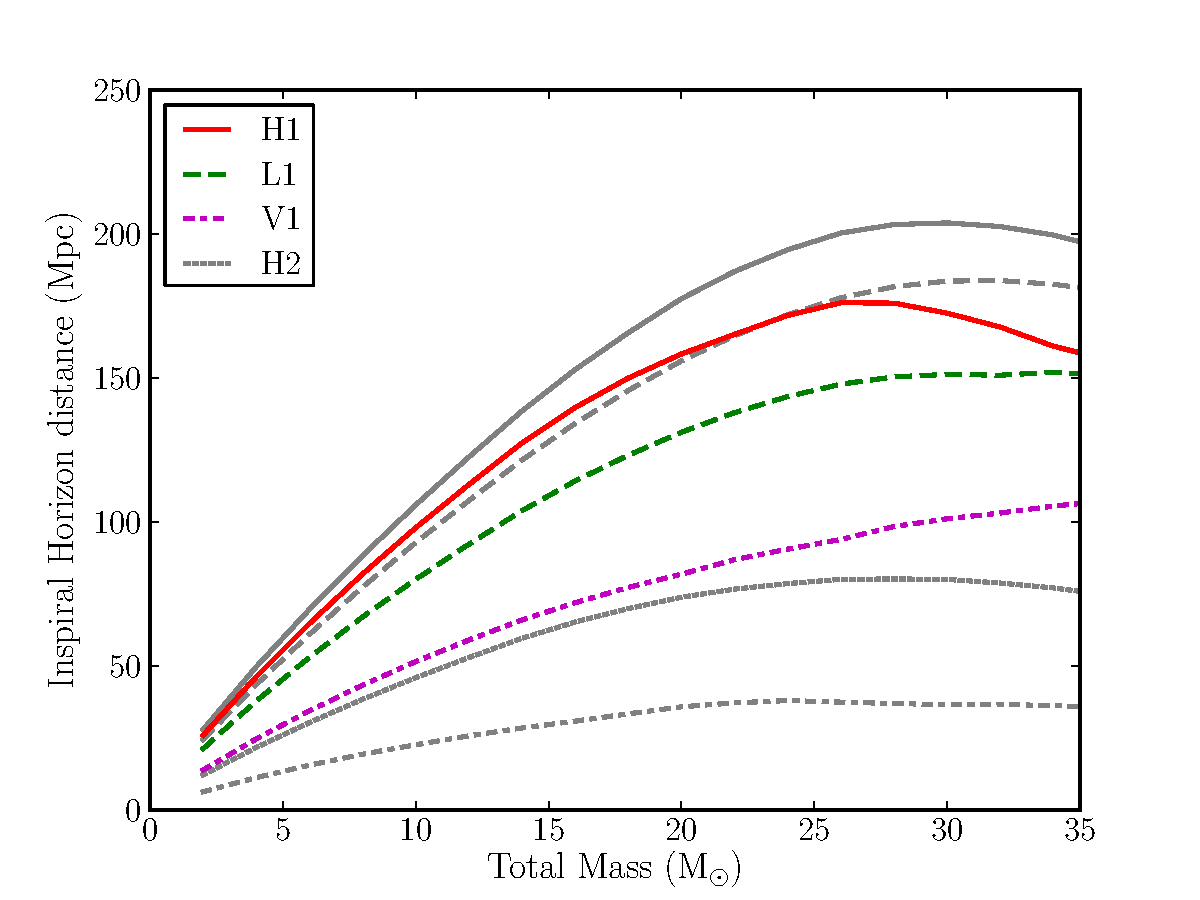
\includegraphics[width=6in]{figures/s6a_insprange.pdf}
\end{center}
\caption{Average inspiral range of S6A. Ranges were computed by \texttt{lalapps\_tmpltbank} using equation \ref{eqn:DtoRho} with $\rho=8$, then averaged over all analysis chunks in the epoch. S6 ranges are in color; best S5 ranges are in gray. Although H2 was not used in \ac{S6}, it is shown for comparison to V1.}
\end{figure}

\begin{figure}[p]
\begin{center}
\label{fig:s6b_pre-hepi_insprange}
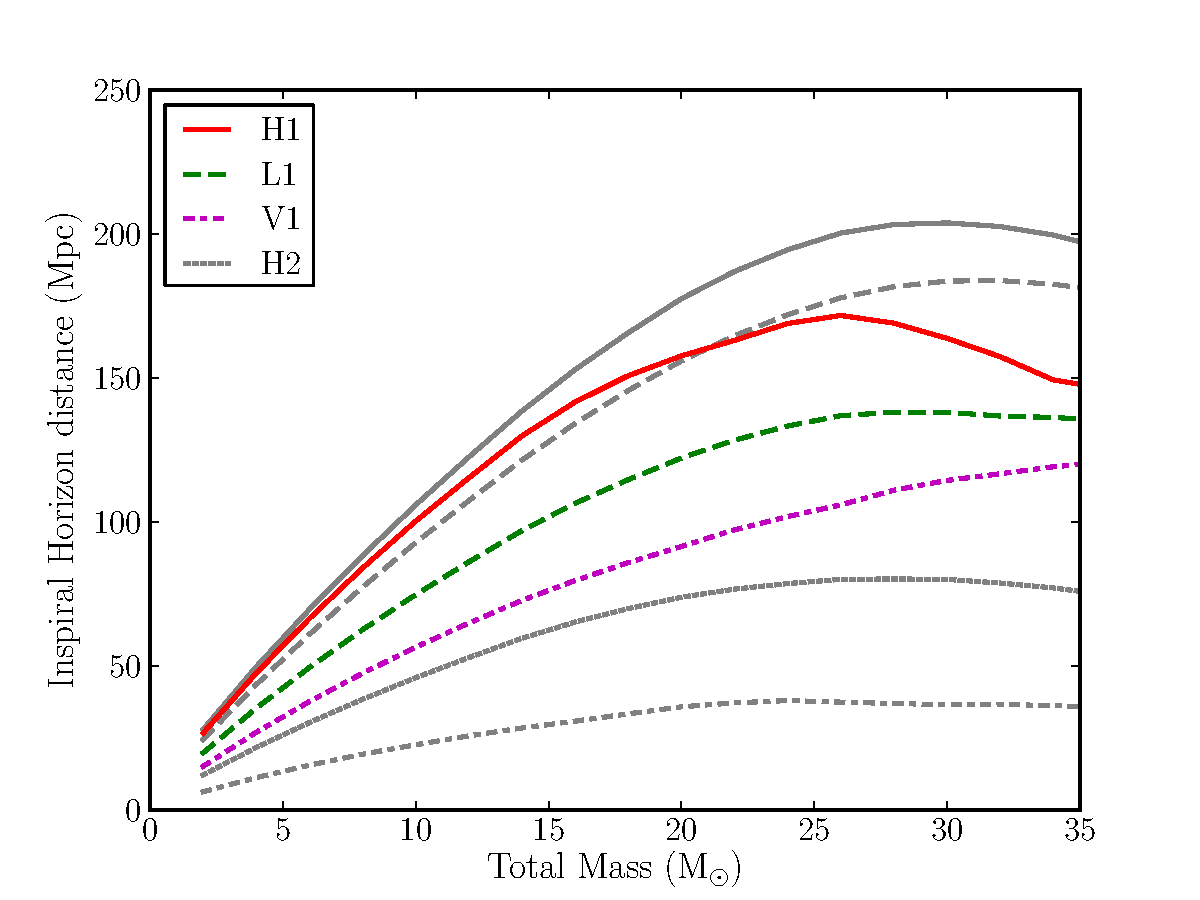
\includegraphics[width=6in]{figures/s6b_pre-hepi_insprange.pdf}
\end{center}
\caption{Average inspiral range of S6B prior to the implementation of \ac{HEPI}. Ranges were computed using the same method as in Figure \ref{fig:s6a_insprange}.}
\end{figure}

\begin{figure}[p]
\begin{center}
\label{fig:s6b_post-hepi_insprange}
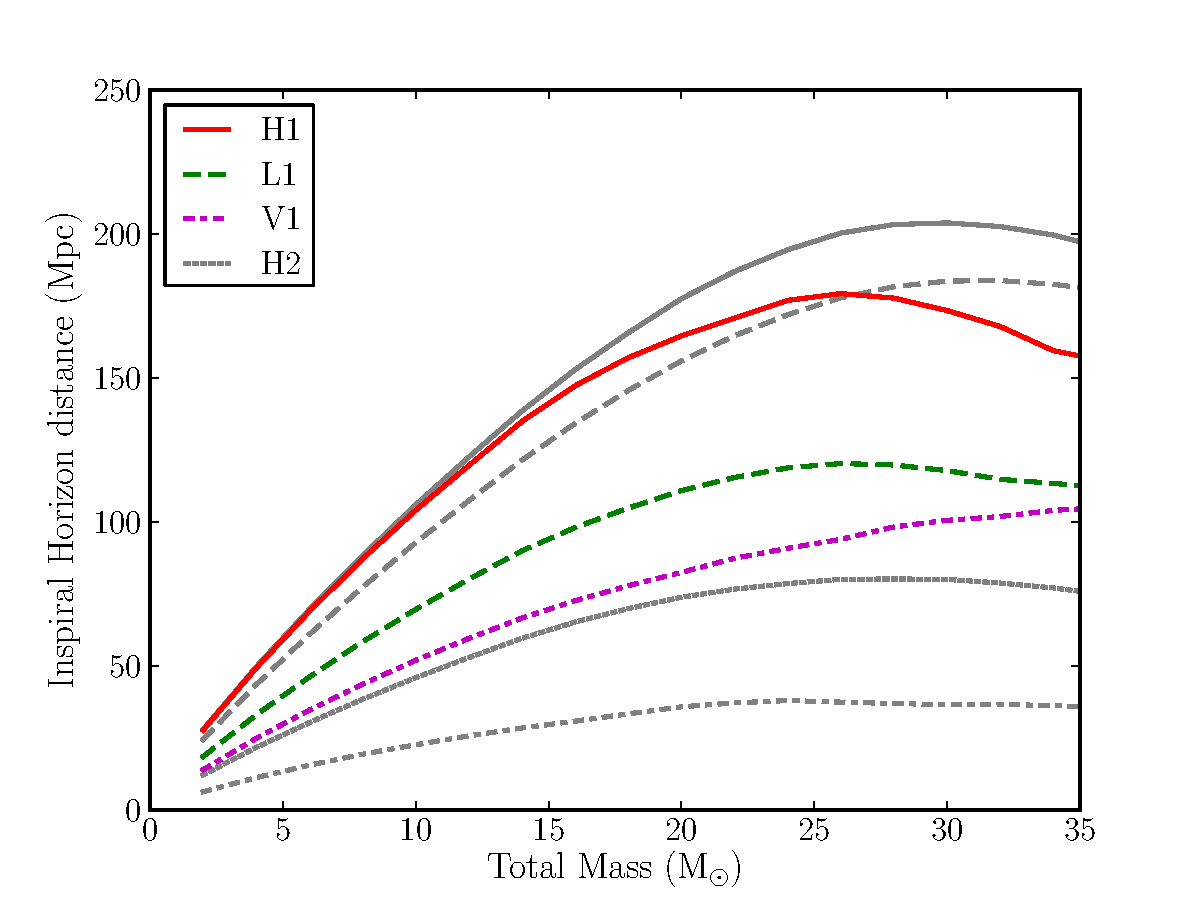
\includegraphics[width=6in]{figures/s6b_post-hepi_insprange.pdf}
\end{center}
\caption{Average inspiral range of S6B after the implementation of \ac{HEPI}. Ranges were computed using the same method as in Figure \ref{fig:s6a_insprange}.}
\end{figure}

\begin{figure}[p]
\begin{center}
\label{fig:s6c_insprange}
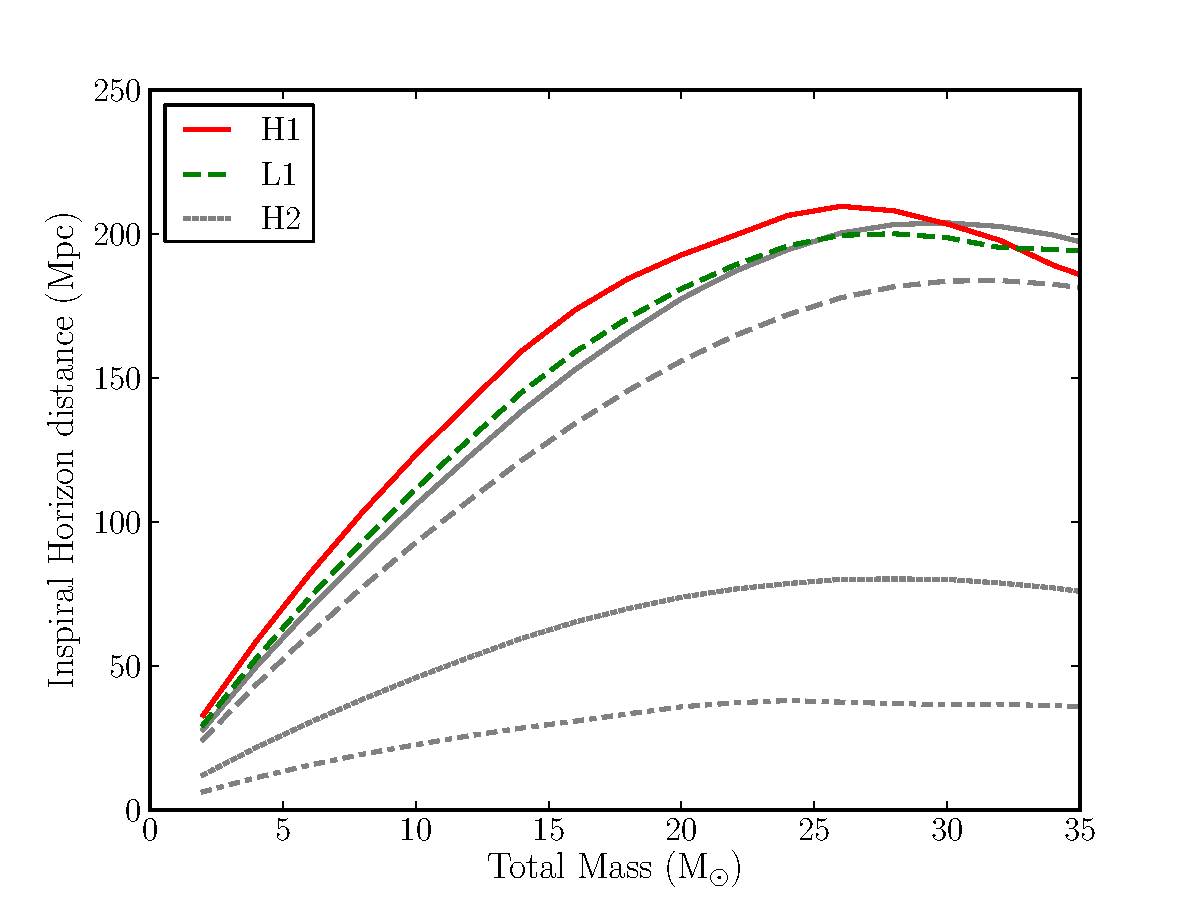
\includegraphics[width=6in]{figures/s6c_insprange.pdf}
\end{center}
\caption{Average inspiral range of S6C. V1 is not shown as it was down for commissioning during this period. Ranges were computed using the same method as in Figure \ref{fig:s6a_insprange}.}
\end{figure}

\begin{figure}[p]
\begin{center}
\label{fig:s6d_insprange}
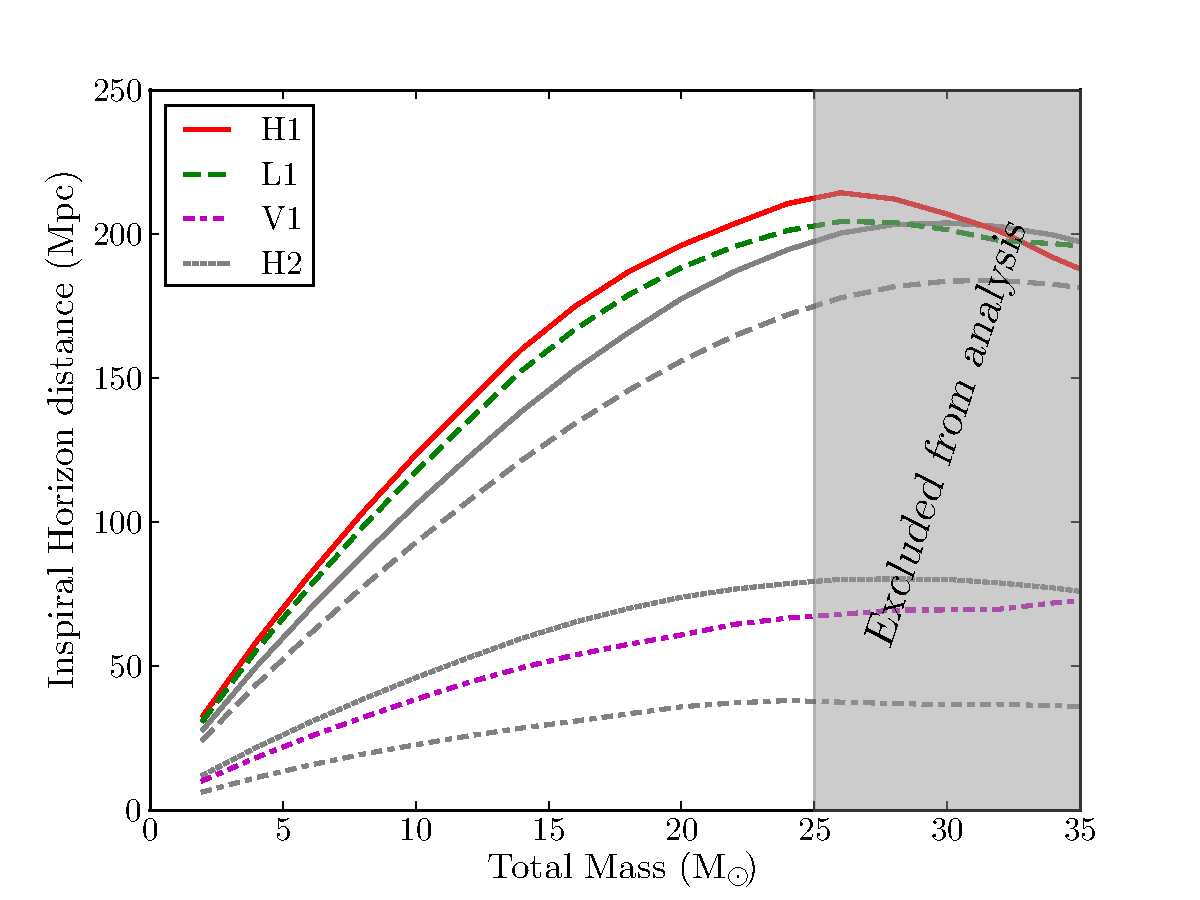
\includegraphics[width=6in]{figures/s6d_insprange_alt.pdf}
\end{center}
\caption{Average inspiral range of S6D. Shaded region indicates the mass range that was excluded in the low mass search for this period. Ranges were computed using the same method as in Figure \ref{fig:s6a_insprange}.}
\end{figure}
